\documentclass{article}
\usepackage{graphicx}
\usepackage[margin=1.5cm]{geometry}
\usepackage{amsmath}

\begin{document}

\title{Thursday Reading Assessment: Unit 2, Ohm's Law, Resistors in Complex Circuits}
\author{Prof. Jordan C. Hanson}

\maketitle

\section{Memory Bank}

\begin{itemize}
\item $R_{tot} = R_1 + R_2$ ... Total resistance of two resistors in series.
\item $R_{tot}^{-1} = R_1^{-1} + R_2^{-1}$ ... Total resistance of two resistors in parallel.
\item $P = IV$ ... The power consumed by a device that draws a current $I$ at a voltage $V$.
\item $\Delta Q = I \Delta t$ ... The definition of current implies that a \textbf{charge} is a current multiplied by a time.
\end{itemize}

\section{Current from Resistance and Voltage}

\begin{enumerate}
\item (a) Suppose an electrical circuit is comprised of a 5V battery, and two 1k$\Omega$ resistors \textit{in series}.  What is the current flowing from the battery? (b) Suppose an electrical circuit is comprised of a 5V battery, and two 1k$\Omega$ resistors \textit{in parallel}.  What is the current flowing from the battery? (c) Compute the power consumption for the circuits in parts (a) and (b).  (d) If the battery has 10 A hr of charge, how long will the battery last in each case? \\ \vspace{2cm}
\end{enumerate}

\section{Kirchhoff's Rules}

\begin{enumerate}
\item Consider the circuit in Fig. \ref{fig:circ}. How long will the battery power the circuit?
\end{enumerate}

\begin{figure}[hb]
\centering
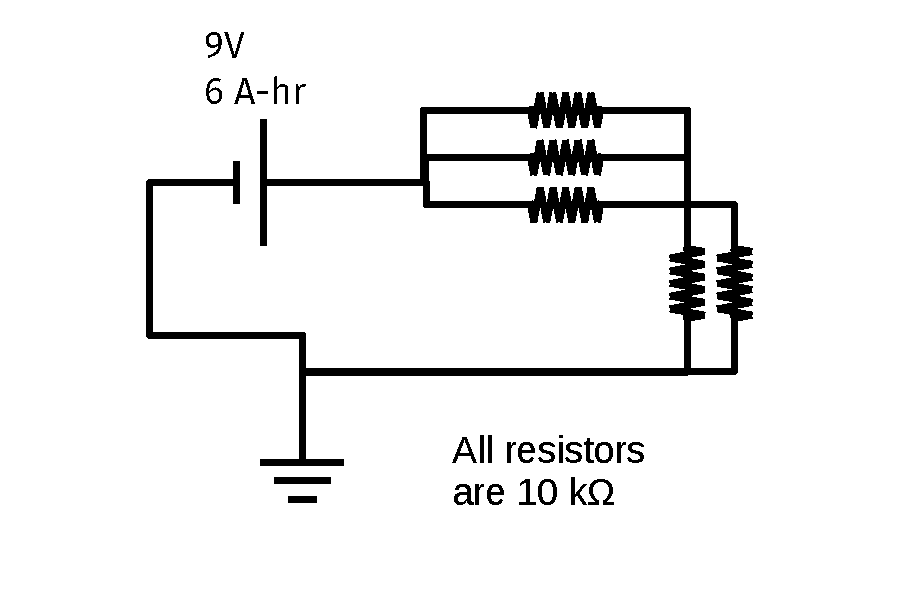
\includegraphics[width=0.5\textwidth,trim=0cm 1.0cm 0cm 1cm,clip=true]{figures/circuitExample1.pdf}
\caption{\label{fig:circ} A circuit with 5 resistors, each with $R=10$ k$\Omega$.}
\end{figure}

\end{document}
